\documentclass[11pt,a4paper]{article}
\usepackage[margin=2.3cm]{geometry}
\usepackage[T1]{fontenc}
\usepackage{lmodern}
\usepackage{amsmath}
\usepackage{booktabs}
\usepackage{graphicx}
\usepackage{multirow}
\usepackage[hidelinks]{hyperref}
\usepackage[font=small,labelfont=bf]{caption}

\newcommand{\F}{\textsf{F}}
\newcommand{\C}{\textsf{C}}
\newcommand{\Lo}{\textsf{L}}

\title{Frozen, Fine-Tuned or From Scratch?\\[2pt]
\large Comparing image encoders for measuring nanoparticles in liquid-phase TEM video}
\author{Nikola Jankovikj\\ Applied Machine Learning --- course project}
\date{November 2026}

\begin{document}
\maketitle

\begin{abstract}
Liquid-phase transmission electron microscopy (LPTEM) films nanoparticles as they move
and grow in liquid, but the frames are noisy and the quantities of interest --- how many
particles there are, how large they are, where they are --- must be read off by a
model. We ask which image encoder reads them best when the reading heads, the loss, the
data and the training budget are held fixed: a frozen self-supervised video model
(V-JEPA~2, ViT-L), the same model adapted with low-rank adapters (LoRA), or a small
convolutional network trained from scratch. On 2000 simulated LPTEM videos with an exact
answer key, and at 10, 30 and 100\,\% of the training data, the frozen encoder is the
weakest on every measure. LoRA and the CNN tie with the full training set (count
$R^2$ 0.843 vs 0.838); with 160 training videos LoRA leads clearly (0.726 vs 0.661)
and matches what the frozen encoder reaches with ten times the data. Particle tracking
is close to its ceiling for all three. Five predictions were written down before any
result; three held.
\end{abstract}

\section{Introduction}

My master's thesis asks whether a self-supervised video model can \emph{predict} how
nanoparticles evolve in LPTEM video: whether a model trained only to predict its own
latent representation of future frames captures growth laws such as $r \propto t^{1/3}$.
An earlier stage of that work found the forecasts limited less by the predictor than by
the \emph{reading} of the frames: the probes that turn V-JEPA~2's frozen features into
particle counts and radii make errors of almost a pixel, which is large next to the
radius changes the growth laws imply.

This project isolates that reading step and asks a standard applied-ML question about
it: \emph{given a fixed task, data set and budget, which encoder should one use?} Three
options span the usual choices:
\begin{itemize}
  \item \F{} --- the pretrained encoder, \textbf{frozen}; only the reading heads are trained.
  \item \Lo{} --- the same encoder \textbf{adapted with LoRA}~\cite{hu2022lora}: small
        low-rank updates to its attention layers, trained together with the heads.
  \item \C{} --- a small \textbf{CNN trained from scratch}, with no pretraining at all.
\end{itemize}
Everything except the encoder is shared, and each model is trained on 10, 30 and
100\,\% of the training videos, so the comparison also measures how much pretraining is
worth when labels are scarce.

\section{Data}

Real LPTEM video with ground truth for every particle does not exist, so the data are
simulated. The \emph{dynamics-v1} set has 2000 videos of 100 frames at
$512\times512$ pixels. Each video follows one of five processes: diffusion-limited
growth ($r\propto t^{1/3}$), reaction-limited growth ($r\propto t^{1/2}$), Ostwald
ripening, coalescence, or no growth (static); particles also undergo Brownian motion with
a known diffusion coefficient $D$ and a slow stage drift. The frames are produced by a
re-implementation of the image formation of the LPTEMsimulator~\cite{lptemsim}:
Beer--Lambert attenuation through gold, water and silicon nitride, a bulging liquid
cell, Poisson shot noise at a given electron dose, and the detector's blur.

Videos come in two strata: \emph{physics} (1600 videos; 6--16 particles of 8--22\,px, dose 6--75 electrons per pixel) and \emph{experiment} (400 videos; imaging
conditions matched to published real video). All results are reported on the
\textbf{physics stratum}, where the ground truth is cleanest; detection and tracking
numbers use all test videos. Every model sees the central $256\times256$ crop.

The unit of input is a \emph{tubelet} of two consecutive frames, the unit V-JEPA~2
encodes; a 100-frame video gives 50 tubelets. For each tubelet the targets are the
\textbf{particle count}, the \textbf{mean radius} and the \textbf{total area} of the
visible particles, plus each particle's position on a $16\times16$ grid of cells.
Videos are split 80/10/10 into train, validation and test \emph{by video} (1600 / 200 /
200, fixed seed), so no test video contributes a single frame to training.

\section{Method}

\subsection{Encoders}

All three encoders map a tubelet to a $16\times16$ grid of tokens, one per
$16\times16$-pixel cell.

\paragraph{\F{}: frozen V-JEPA 2.} V-JEPA~2~\cite{assran2025vjepa2} is a ViT-L
(304\,M parameters, token width 1024) pretrained with a self-supervised objective:
predicting the representation of masked parts of a video from the visible parts. Its
weights are not touched; the tokens were computed once and cached.

\paragraph{\Lo{}: V-JEPA 2 + LoRA.} The same network, frozen, with rank-16 LoRA updates
($\alpha=32$) on the query, key, value and output projections of all 24 attention
layers (\texttt{peft}~\cite{peft}). At initialisation LoRA is the identity, and we
checked that \Lo{}'s tokens equal \F{}'s (cosine similarity 1.00000), so \Lo{} starts
exactly where \F{} is. The adapters add 3.1\,M trainable parameters.

\paragraph{\C{}: CNN from scratch.} Four blocks, each a stride-2 $3\times3$
convolution followed by a $3\times3$ convolution, with batch normalisation and ReLU
(channels 32, 64, 128, 256): the two frames are the two input channels, and four halvings
take $256\times256$ pixels to the same $16\times16$ grid. It has 1.2\,M parameters and no
pretraining.

\subsection{Heads, loss and training}

The heads are the same for all three (only their width follows the encoder's token
width):
\begin{itemize}
  \item an \textbf{attentive probe}: one learned query cross-attends over the 256 tokens
        and a linear layer outputs count, mean radius and total area;
  \item a \textbf{centroid probe}: per token, the logit that a particle centre lies in
        that cell and the centre's sub-cell offset.
\end{itemize}
The loss is the sum of the mean-squared error of the three observables (each
standardised with training-set statistics), a positively weighted binary cross-entropy
on cell occupancy (about 5\,\% of cells are occupied), and the squared offset error on
occupied cells. Optimisation is AdamW, batch 32, learning rate $10^{-3}$ for heads and
the CNN and $10^{-4}$ for the LoRA adapters.

\paragraph{Equal budgets.} Training subsets are nested (the 10\,\% subset is inside the
30\,\% subset, which is inside the full set) and identical across models, and every
model sees the same number of training samples at every fraction: with $1/10$ of the
data it trains for $10\times$ the epochs (Table~\ref{tab:budget}). \C{} and \Lo{} keep
the checkpoint with the lowest validation loss; \F{} trains for a fixed number of epochs,
the protocol of the earlier thesis stage.

\begin{table}[t]
\centering\small
\begin{tabular}{lllc}
\toprule
& encoder & trainable parameters & epochs at 100 / 30 / 10\,\% \\
\midrule
\F{} & V-JEPA 2 ViT-L, frozen & 4.5\,M (heads) & 50 / 167 / 500 \\
\Lo{} & V-JEPA 2 ViT-L + LoRA & 7.6\,M (3.1\,M adapters + heads) & 6 / 20 / 60 \\
\C{} & 4-block CNN & 1.5\,M (1.2\,M CNN + heads) & 20 / 67 / 200 \\
\bottomrule
\end{tabular}
\caption{The three models. Heads on the 1024-wide V-JEPA tokens are larger than on the
CNN's 256-wide tokens, so \F{} trains more parameters than the whole CNN. \Lo{}'s epoch
count was set from a one-epoch timing run; one run on an RTX 3090 took 1.7--2.7\,h for
\Lo{}, 12--17\,min for \C{}.}
\label{tab:budget}
\end{table}

\subsection{Evaluation}

\begin{itemize}
  \item \textbf{$R^2$} of count, mean radius and total area over all test tubelets.
  \item \textbf{Radius reading error}: the mean absolute error of the mean radius on
        tubelets that contain a particle, divided by 0.80 to express it as the standard
        deviation of equivalent Gaussian noise (the quantity the thesis's growth analysis
        uses). It is reported overall and split at a beam dose of 21.2 electrons per pixel
        into \emph{low} and \emph{high} dose.
  \item \textbf{Detection}: occupancy thresholded at the value that maximises F1 on the
        validation set; precision, recall and F1 on test.
  \item \textbf{Tracking}: detections are linked into trajectories with
        trackpy~\cite{trackpy}, and the mean squared displacement gives an estimate of
        $D$. We report the ratio of the estimated to the true $D$, next to the ratio a
        \emph{perfect} detector reaches with the same linking (0.955).
\end{itemize}
Uncertainty is a 95\,\% bootstrap confidence interval that resamples whole test videos
(2000 draws), since tubelets of one video are not independent. All models are resampled
with the \emph{same} draws, so differences between models are paired.

\subsection{Predictions}

Before any of the runs, the following predictions were written into the project plan:
\begin{enumerate}
  \item \C{} $\ge$ \F{} on count with all the data: finding blobs is what CNNs are
        good at.
  \item \F{} $>$ \C{} on count and mean radius with 10\,\% of the data: pretraining
        should pay when labels are few.
  \item \Lo{} $\ge$ \F{} and \Lo{} $\ge$ \C{} on every $R^2$ with all the data.
  \item \Lo{}'s radius reading error is below \F{}'s, but by less than half; the
        low-dose penalty shrinks but remains.
  \item All three estimate $D$ within 10\,\% of the perfect-detector ceiling.
\end{enumerate}

\section{Results}

\begin{table}[t]
\centering\small
\begin{tabular}{llccc}
\toprule
data & model & count $R^2$ & mean radius $R^2$ & total area $R^2$ \\
\midrule
\multirow{3}{*}{100\,\%} & \F{} & 0.726 {\scriptsize[0.665, 0.774]} & 0.902 {\scriptsize[0.876, 0.922]} & 0.928 {\scriptsize[0.914, 0.941]} \\
& \C{} & 0.838 {\scriptsize[0.802, 0.865]} & 0.950 {\scriptsize[0.936, 0.961]} & \textbf{0.978} {\scriptsize[0.973, 0.982]} \\
& \Lo{} & \textbf{0.843} {\scriptsize[0.795, 0.877]} & \textbf{0.951} {\scriptsize[0.936, 0.961]} & 0.976 {\scriptsize[0.969, 0.981]} \\
\midrule
\multirow{3}{*}{30\,\%} & \F{} & 0.646 {\scriptsize[0.562, 0.709]} & 0.872 {\scriptsize[0.842, 0.894]} & 0.910 {\scriptsize[0.893, 0.928]} \\
& \C{} & 0.757 {\scriptsize[0.671, 0.821]} & 0.918 {\scriptsize[0.898, 0.933]} & 0.943 {\scriptsize[0.929, 0.955]} \\
& \Lo{} & \textbf{0.781} {\scriptsize[0.731, 0.821]} & \textbf{0.941} {\scriptsize[0.923, 0.955]} & \textbf{0.946} {\scriptsize[0.927, 0.957]} \\
\midrule
\multirow{3}{*}{10\,\%} & \F{} & 0.587 {\scriptsize[0.482, 0.667]} & 0.819 {\scriptsize[0.769, 0.857]} & 0.859 {\scriptsize[0.829, 0.890]} \\
& \C{} & 0.661 {\scriptsize[0.552, 0.745]} & 0.864 {\scriptsize[0.824, 0.894]} & 0.910 {\scriptsize[0.877, 0.941]} \\
& \Lo{} & \textbf{0.726} {\scriptsize[0.652, 0.782]} & \textbf{0.922} {\scriptsize[0.899, 0.938]} & \textbf{0.931} {\scriptsize[0.906, 0.954]} \\
\bottomrule
\end{tabular}
\caption{$R^2$ on the test videos (physics stratum, 158 videos), with 95\,\% bootstrap
intervals. 100\,\% = 1600 training videos.}
\label{tab:r2}
\end{table}

\begin{figure}[t]
\centering
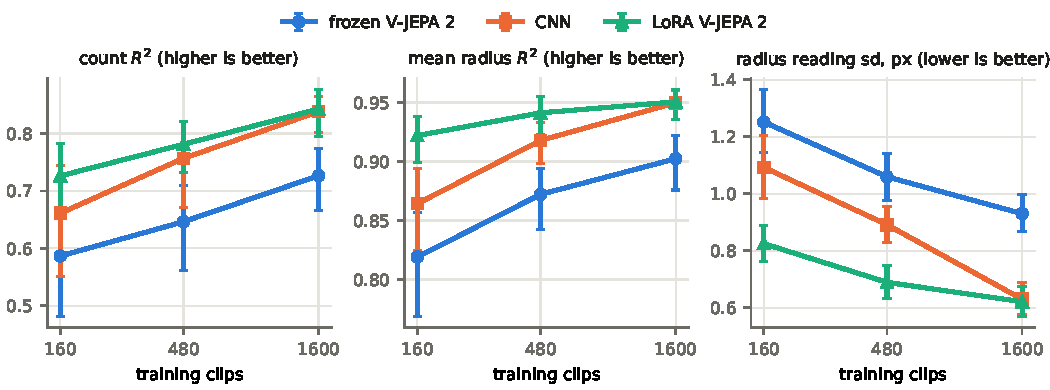
\includegraphics[width=\linewidth]{fig_data_efficiency.pdf}
\caption{The same results against training-set size (log scale), with 95\,\%
intervals. Right: the radius reading error in pixels, where lower is better.}
\label{fig:eff}
\end{figure}

\paragraph{Accuracy (Table~\ref{tab:r2}, Figure~\ref{fig:eff}).} The frozen encoder is
last on all three observables at every data size. With the full training set \Lo{} and
\C{} are tied: their paired differences are $+0.005$, $+0.001$ and $-0.002$, and every
interval contains zero. As data shrink the two separate: at 10\,\% \Lo{} leads \C{} by
0.065 on count and 0.058 on mean radius. \Lo{} with 160 training videos reaches the same
count $R^2$ as \F{} with 1600 (0.726) and a higher mean-radius $R^2$ (0.922 vs 0.902).

\begin{table}[t]
\centering\small
\begin{tabular}{llcccc}
\toprule
data & model & all & low dose & high dose & low $-$ high \\
\midrule
\multirow{3}{*}{100\,\%} & \F{} & 0.93 {\scriptsize[0.87, 1.00]} & 1.06 & 0.83 & 0.23 {\scriptsize[0.11, 0.37]} \\
& \C{} & 0.63 {\scriptsize[0.58, 0.69]} & 0.76 & 0.52 & 0.24 {\scriptsize[0.13, 0.36]} \\
& \Lo{} & \textbf{0.62} {\scriptsize[0.57, 0.67]} & 0.72 & 0.54 & 0.17 {\scriptsize[0.07, 0.29]} \\
\midrule
\multirow{3}{*}{30\,\%} & \F{} & 1.06 {\scriptsize[0.98, 1.14]} & 1.23 & 0.92 & 0.31 {\scriptsize[0.15, 0.49]} \\
& \C{} & 0.89 {\scriptsize[0.83, 0.96]} & 0.99 & 0.81 & 0.18 {\scriptsize[0.05, 0.32]} \\
& \Lo{} & \textbf{0.69} {\scriptsize[0.63, 0.75]} & 0.79 & 0.61 & 0.19 {\scriptsize[0.07, 0.31]} \\
\midrule
\multirow{3}{*}{10\,\%} & \F{} & 1.25 {\scriptsize[1.14, 1.37]} & 1.45 & 1.09 & 0.35 {\scriptsize[0.13, 0.60]} \\
& \C{} & 1.09 {\scriptsize[0.98, 1.20]} & 1.20 & 1.00 & 0.20 {\scriptsize[$-$0.02, 0.42]} \\
& \Lo{} & \textbf{0.83} {\scriptsize[0.76, 0.89]} & 0.93 & 0.74 & 0.19 {\scriptsize[0.07, 0.33]} \\
\bottomrule
\end{tabular}
\caption{Radius reading error (pixels, Gaussian-equivalent standard deviation), overall
and by electron dose.}
\label{tab:sd}
\end{table}

\paragraph{Radius reading error (Table~\ref{tab:sd}).} Adapting the encoder cuts \F{}'s
error by a third, from 0.93 to 0.62\,px; the CNN gets to the same place with all the
data but not with less. Low dose costs every model about 0.2\,px: better encoders lower
both dose bins rather than closing the gap between them.

\begin{table}[t]
\centering\small
\begin{tabular}{lccc}
\toprule
& \F{} & \C{} & \Lo{} \\
\midrule
precision (100 / 30 / 10\,\%) & 0.870 / 0.863 / 0.874 & 0.920 / 0.922 / 0.906 & 0.923 / 0.924 / 0.923 \\
recall & 0.797 / 0.805 / 0.786 & 0.860 / 0.848 / 0.829 & 0.866 / 0.851 / 0.842 \\
F1 & 0.832 / 0.833 / 0.827 & 0.889 / 0.883 / 0.866 & 0.893 / 0.886 / 0.881 \\
estimated $D$ / true $D$ & 0.986 / 0.991 / 1.007 & 0.971 / 0.967 / 0.966 & 0.981 / 0.993 / 1.000 \\
\bottomrule
\end{tabular}
\caption{Detection and diffusion on all test videos. A perfect detector with the same
linking reaches $D$ ratio 0.955.}
\label{tab:det}
\end{table}

\paragraph{Detection and tracking (Table~\ref{tab:det}).} \C{} and \Lo{} detect 5--6
points of F1 better than \F{}. Yet all nine runs estimate the diffusion coefficient
within 6\,\% of what a perfect detector achieves: missed and spurious detections barely
affect the linked trajectories, so positions are not where the encoders differ.

\paragraph{Predictions.}
\begin{enumerate}
  \item \textbf{Right.} \C{} $-$ \F{} on count at 100\,\%: $+0.112$ [0.075, 0.154].
  \item \textbf{Wrong.} At 10\,\% the frozen encoder \emph{loses} to the CNN: $-0.075$
        [$-0.121$, $-0.031$] on count, $-0.045$ [$-0.076$, $-0.020$] on mean radius.
  \item \textbf{Wrong as stated, tied in substance.} \Lo{} beats \F{} on all three
        $R^2$ (intervals above zero) but is tied with \C{}, and its total-area $R^2$ is
        0.002 lower.
  \item \textbf{Right.} 0.62 vs 0.93\,px is a cut of a third, not half; \Lo{}'s low-dose
        penalty (0.17) is below \F{}'s (0.23) and still above zero [0.07, 0.29], although
        the reduction itself is within noise [$-0.16$, $+0.04$].
  \item \textbf{Right.} All $D$ estimates are 1.01--1.06 times the ceiling.
\end{enumerate}

\section{Discussion}

\paragraph{Pretraining helps only once it is adapted.} Prediction 2 had the right
intuition for the wrong model. With few labels, pretraining did pay --- \Lo{} is the best
model at 10\,\% by a wide margin --- but only after the encoder was allowed to change. The
frozen features are not missing the information: \Lo{} starts from exactly \F{}'s tokens
and reaches much better numbers with only 3\,M extra parameters. The features are
general-purpose; the probes cannot extract particle sizes from them as well as a lightly
adapted encoder can, and even a small CNN that learns its features for this task does
better.

\paragraph{With enough data, the simple model is enough.} With 1600 training videos
the 1.2\,M-parameter CNN matches a 304\,M-parameter pretrained transformer on every
observable, at about an eighth of the training time. The practical rule from these
results: if labelled data are plentiful, a small task-specific CNN is the cost-effective
choice; when they are scarce, adapting a pretrained model is clearly better, and using
it frozen is the worst of the three.

\paragraph{Some errors are in the frames.} Every model reads radii about 0.2\,px worse at
low dose, and better encoders do not close that gap. At low dose fewer electrons
reach the detector and particle edges are lost in shot noise; that is a limit of the
images, not of the encoder.

\paragraph{For the thesis.} The plan fixed in advance that the growth forecasts would be
repeated with \Lo{}'s features only if \Lo{}'s reading error fell to 0.6\,px or below.
It is 0.621\,px [0.571, 0.674]: just above the line, with an interval that straddles it.
By the rule as written the rerun is not triggered; any decision to run it anyway is made
after seeing this result and will be reported as such.

\section{Limitations}

\begin{itemize}
  \item \textbf{One training seed per run.} The intervals cover which videos are in the
        test set, not training randomness; the \Lo{}--\C{} tie at 100\,\% and the
        0.6\,px threshold would need repeated seeds to settle.
  \item \textbf{Different stopping rules.} \C{} and \Lo{} keep their best-validation
        epoch, \F{} trains for a fixed number of epochs. \C{} and \Lo{} overfit within a
        few epochs (best epochs 3--7) and depend on that checkpoint; \F{}'s training loss
        levels off instead, so it probably loses little from the fixed schedule.
  \item \textbf{Detection and tracking have no intervals}, and the localisation error in
        pixels was not computed, because the predicted positions were not saved.
  \item \textbf{Synthetic data only.} The simulator's imaging conditions bracket
        published real video, but the comparison has not been repeated on real movies.
\end{itemize}

\section{Conclusion}

For reading nanoparticle counts and sizes from LPTEM video, a frozen self-supervised
video encoder is the weakest of the three options at every data size. Adapting it with
LoRA makes it the best option when labels are scarce, matching the frozen encoder with a
tenth of the data; with plenty of labels, a small CNN trained from scratch does just as
well. Particle tracking is near its ceiling for all three, and low electron dose costs
every encoder the same.

\paragraph{Reproducibility.} Code, run metrics and per-video predictions are in the
project repository:
\begin{itemize}
  \item training: \texttt{scripts/train\_encoder\_compare.py};
  \item every number in this report: \texttt{scripts/encoder\_compare\_report.py};
  \item results: \texttt{experiments/encoder-compare/}.
\end{itemize}

\begin{thebibliography}{9}
\bibitem{assran2025vjepa2} M.~Assran et al.
  \newblock V-JEPA 2: Self-supervised video models enable understanding, prediction and
  planning. \newblock arXiv:2506.09985, 2025.
\bibitem{hu2022lora} E.~J.~Hu et al.
  \newblock LoRA: Low-rank adaptation of large language models.
  \newblock In \emph{ICLR}, 2022.
\bibitem{peft} S.~Mangrulkar et al.
  \newblock PEFT: State-of-the-art parameter-efficient fine-tuning methods.
  \newblock \url{https://github.com/huggingface/peft}, 2022.
\bibitem{lptemsim} Jamali Lab.
  \newblock LPTEMsimulator. \newblock \url{https://github.com/JamaliLab/LPTEMsimulator}.
\bibitem{trackpy} D.~B.~Allan, T.~Caswell, N.~C.~Keim, C.~M.~van~der~Wel, R.~W.~Verweij.
  \newblock trackpy: Fast, flexible particle-tracking toolkit.
  \newblock Zenodo, \url{https://github.com/soft-matter/trackpy}.
\end{thebibliography}

\end{document}
